\section{Proof of Concepts}

One main part of the investigation into the CERN-Solid collaboration is the development of a \gls{poc}. The \gls{poc} contains the creation of two independent software modules in an existing system from \gls{cern}. These software modules should show how it is to develop with the Solid principles in mind and to the Solid standard.

The goal of these modules is the symbiosis of decentralized stored data in a highly functional system without comprising its performance, security, or usability.

\subsection{POC 1: Commenting Module for Events in Indico}

The first \gls{poc} is supposed to enrich the Indico system with some sort of Solid-based content. With the product owner and chief developer of Indico, the CERN-Solid project manager and a Solid developer it was decided a commenting module for Indico events is an adequate solution to include data from an external storage entity namely a Solid pod. The ability to allow users of Indico to leave a comment on an event, which then lives in a Solid pod completely controlled by the author of the comment was concluded to be an attractive feature for Indico.

\begin{figure}
    \centering
    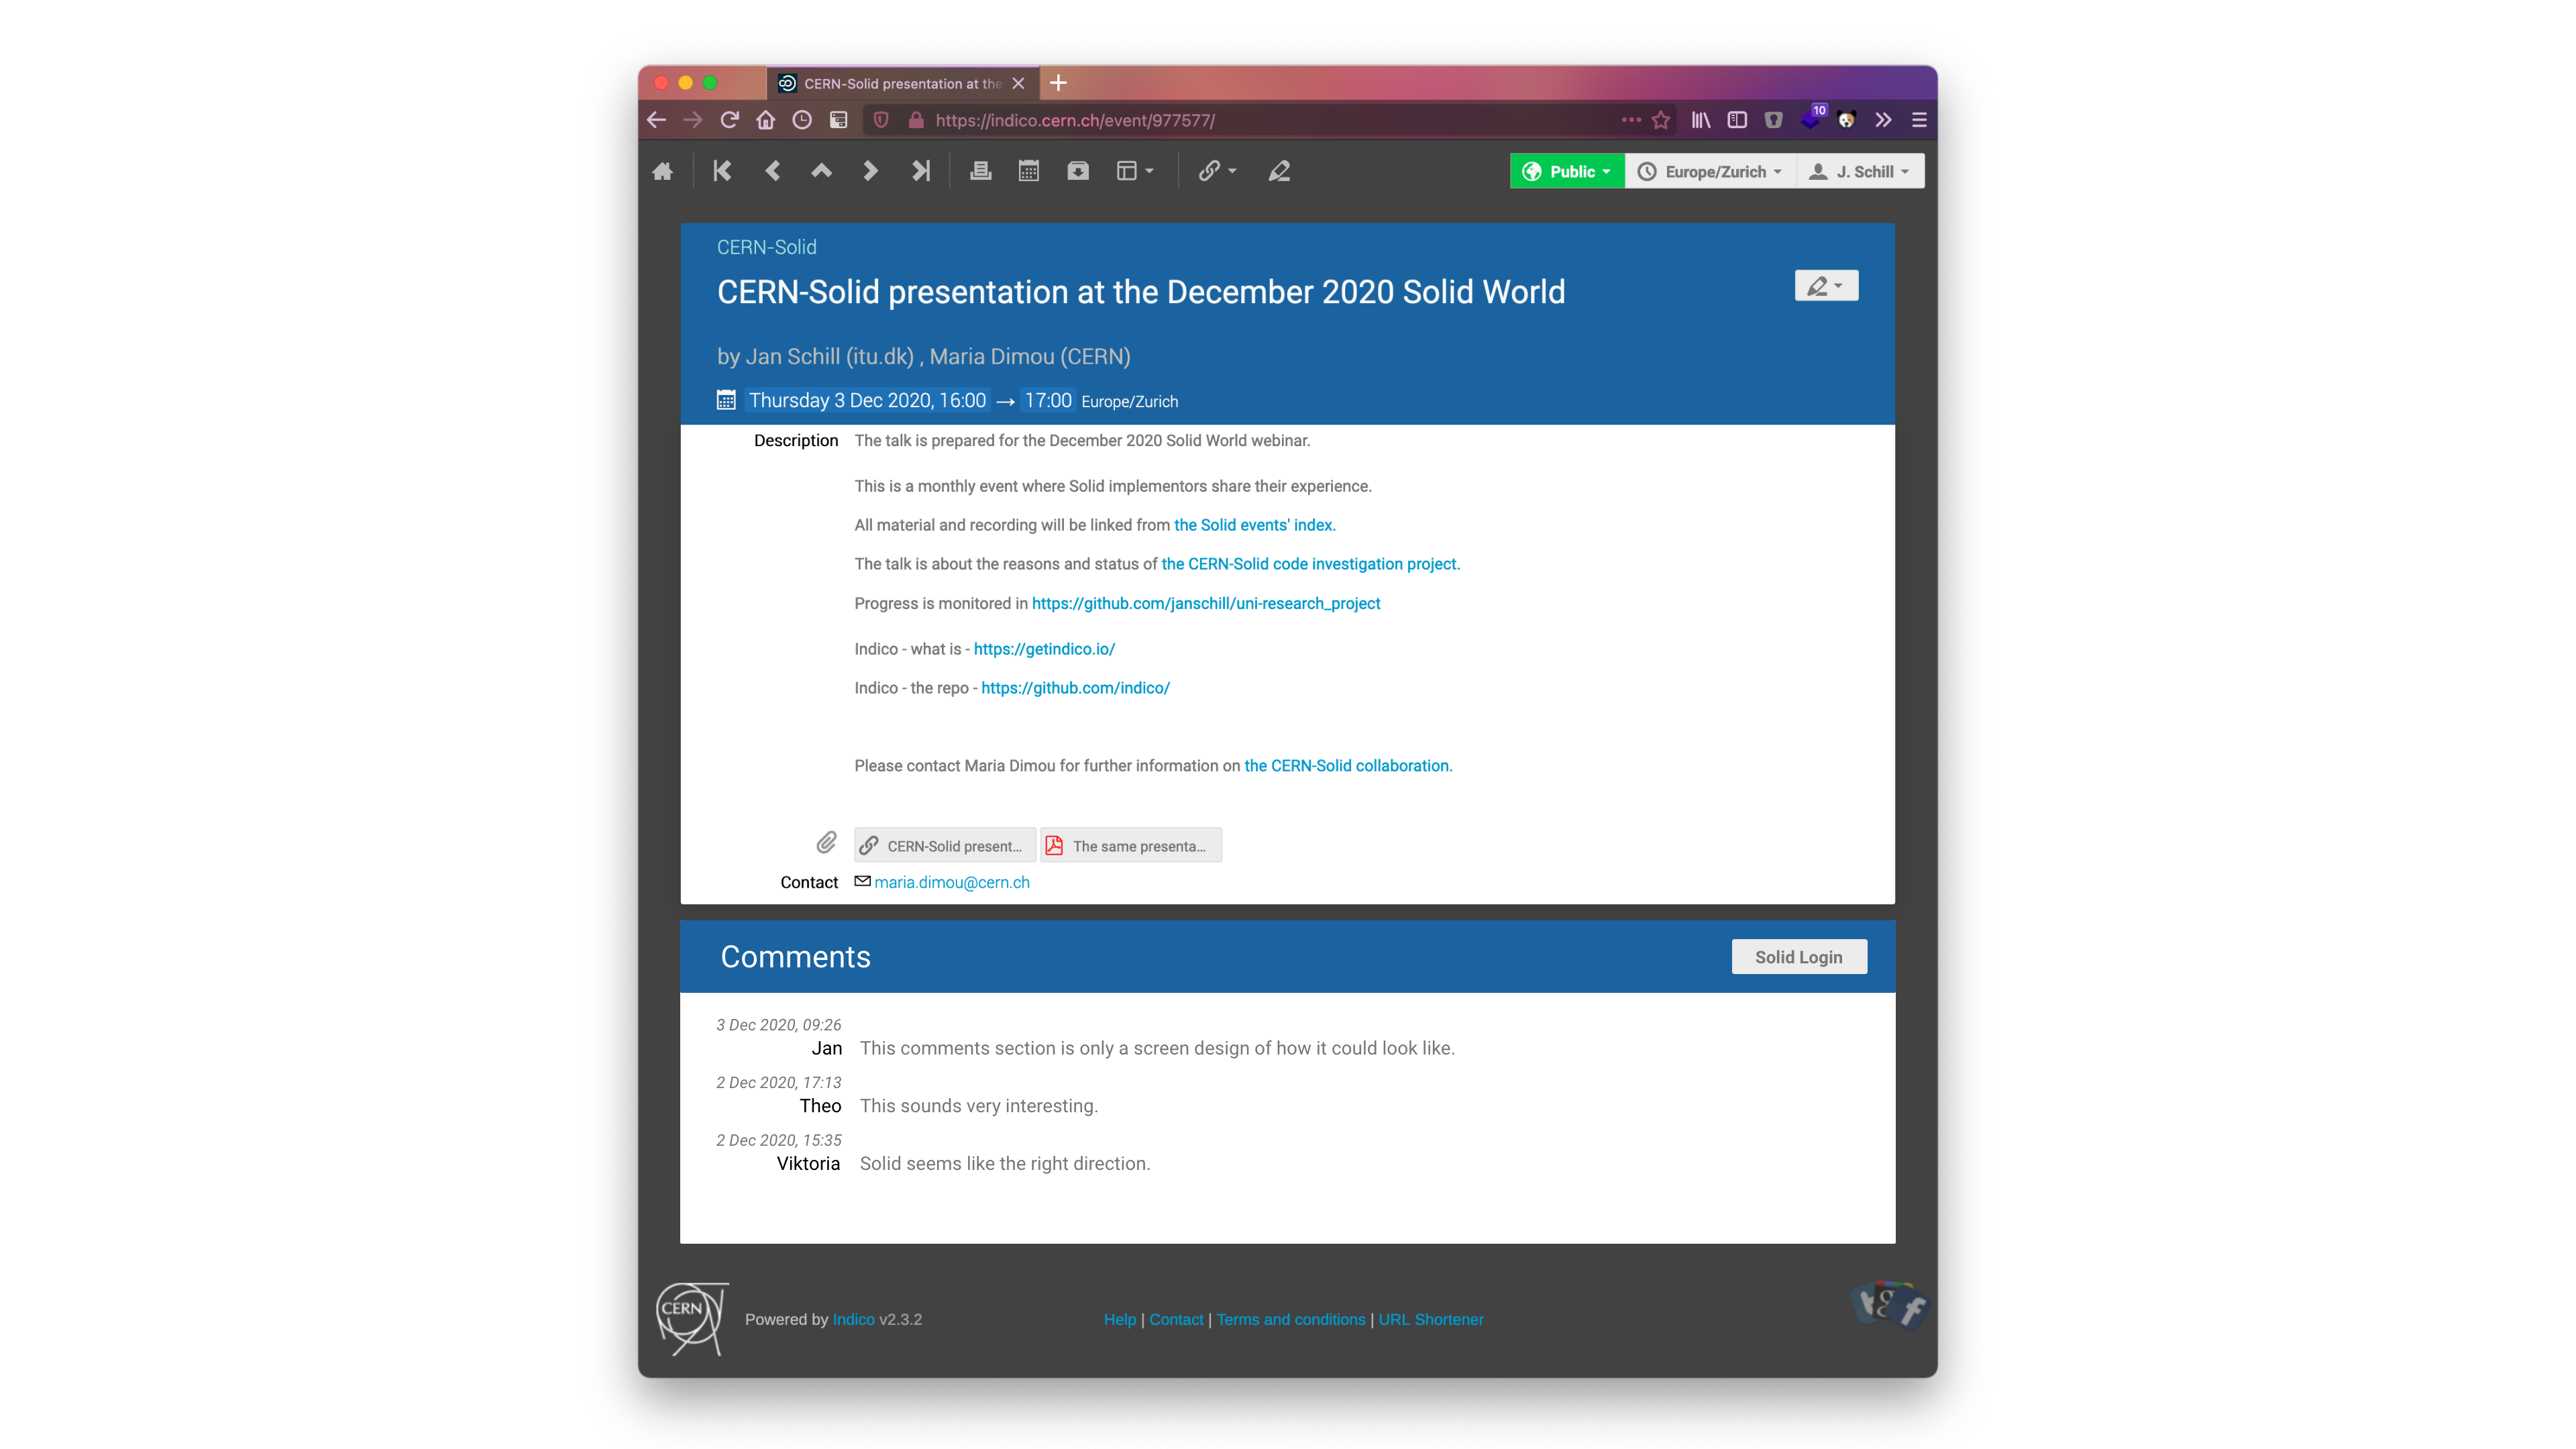
\includegraphics[width=1\textwidth]{prototype/screen_design/indico-comments-screen_design.png}
    \caption{User interface showing the comment module.}
    \label{fig:indico-comments-screen_design}
\end{figure}

\subsubsection{Design}\mbox{}\\

For the implementation of this module several design decisions had to be made. From the fundamental choice of the module running on the client device or be computed on the server and then propagated to the client afterwards or even with a microservice proxying all traffic through it to enable Solid without changing Indico.
Other design challenges were around how to protect the resources holding the comment information. These resources reside on the external Solid pod and need to be fetched from the application and read by other agents. Can \glspl{acl} be configured to allow the specific use-case?

\paragraph{Client- versus Server-Side versus Microservice}\mbox{}\\

When an agent browses to a running instance of Indico most of the functionality is being prepared on the server hosting Indico. It retrieves the specific request, builds the \gls{html}, and sends it to the user. For Indico most of the functionality is built with Python and the web framework Flask. Sometimes functionality needs to be closer to the user, an example is dynamic rendering of \gls{dom} elements. This is useful when new data needs to be shown right away without getting the blank white screen on a page reload.
Indico does send JavaScript, which is used for client-side features, but it focuses on keeping most its features on the server.

To make the right decision if the module should be primarily developed for the client- or server-side or even as a microservice, a list of requirements to the module had to be defined. With the defined requirements in place it had to be figured out how much functionality can be extracted from existing libraries and how much needed to be implemented with the new module. Implementing existing functionality for a new programming language would defeat the \gls{poc}’s purpose of showing how an existing software could work with the Solid principles.

The rudimentary set of features to enable commenting for users in Indico while saving the data in a Solid pod includes: 

\begin{enumerate}
    \item Authentication with a Solid \gls{idp}
    \item (Authenticated) Requests to a Solid pod
    \item Parsing of structured data (Linked Data)
\end{enumerate}

\paragraph{Client Approach}\mbox{}\\

The module runs in the browser and is therefore written in JavaScript. A programming language which compiles to JavaScript, such as TypeScript, is also possible. This means Indico remains mostly untouched, but would have to serve the needed JavaScript to the client on traffic to an event endpoint where the comment module is integrated.

\begin{table}[h!]
    \centering
    \begin{tabular}{c | c} 
     Problem & Solution \\
     \hline
      Language & JavaScript or TypeScript  \\
      Framework & Native JavaScript  \\
      Client & solid-client-js \cite{solid-client-js}  \\
      Authentication & solid-client-authn-browser \cite{solid-client-authn-browser} \\
      RDF & solid-common-vocab-js \cite{solid-common-vocab-js}, rdflib.js \cite{rdflib.js}  \\
    \end{tabular}
    \vspace{0.75cm}
    \caption{Table to test captions and labels}
    \label{table:1}
\end{table}

The communication flow with the Solid Pod of the module would TODO:

\begin{figure}
    \centering
    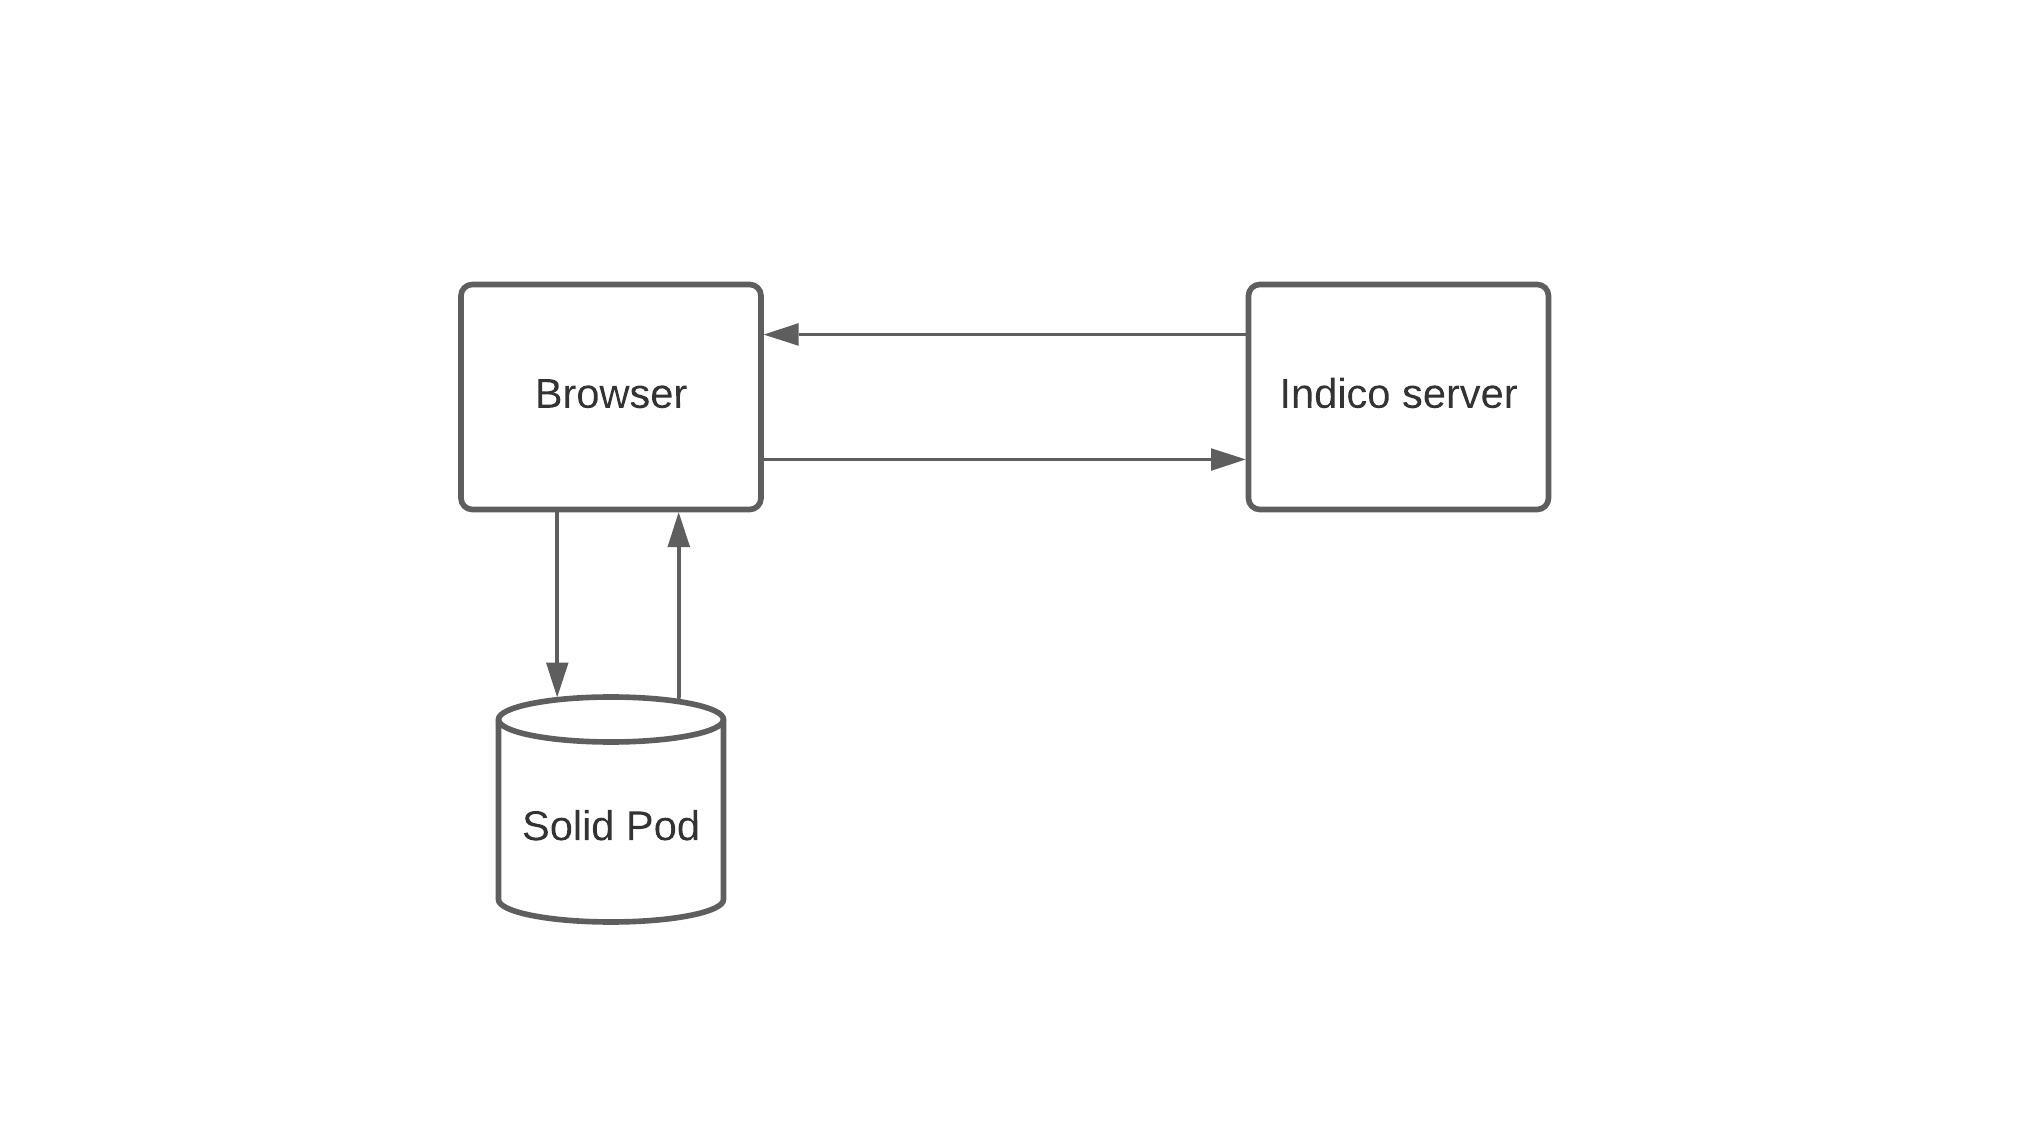
\includegraphics[width=0.8\textwidth]{prototype/graphs/poc-infrastructure-frontend.jpeg}
    \caption{Communication flow for a module developed on the client.}
    \label{fig:poc-infrastructure-frontend}
\end{figure}

\begin{figure}
    \centering
    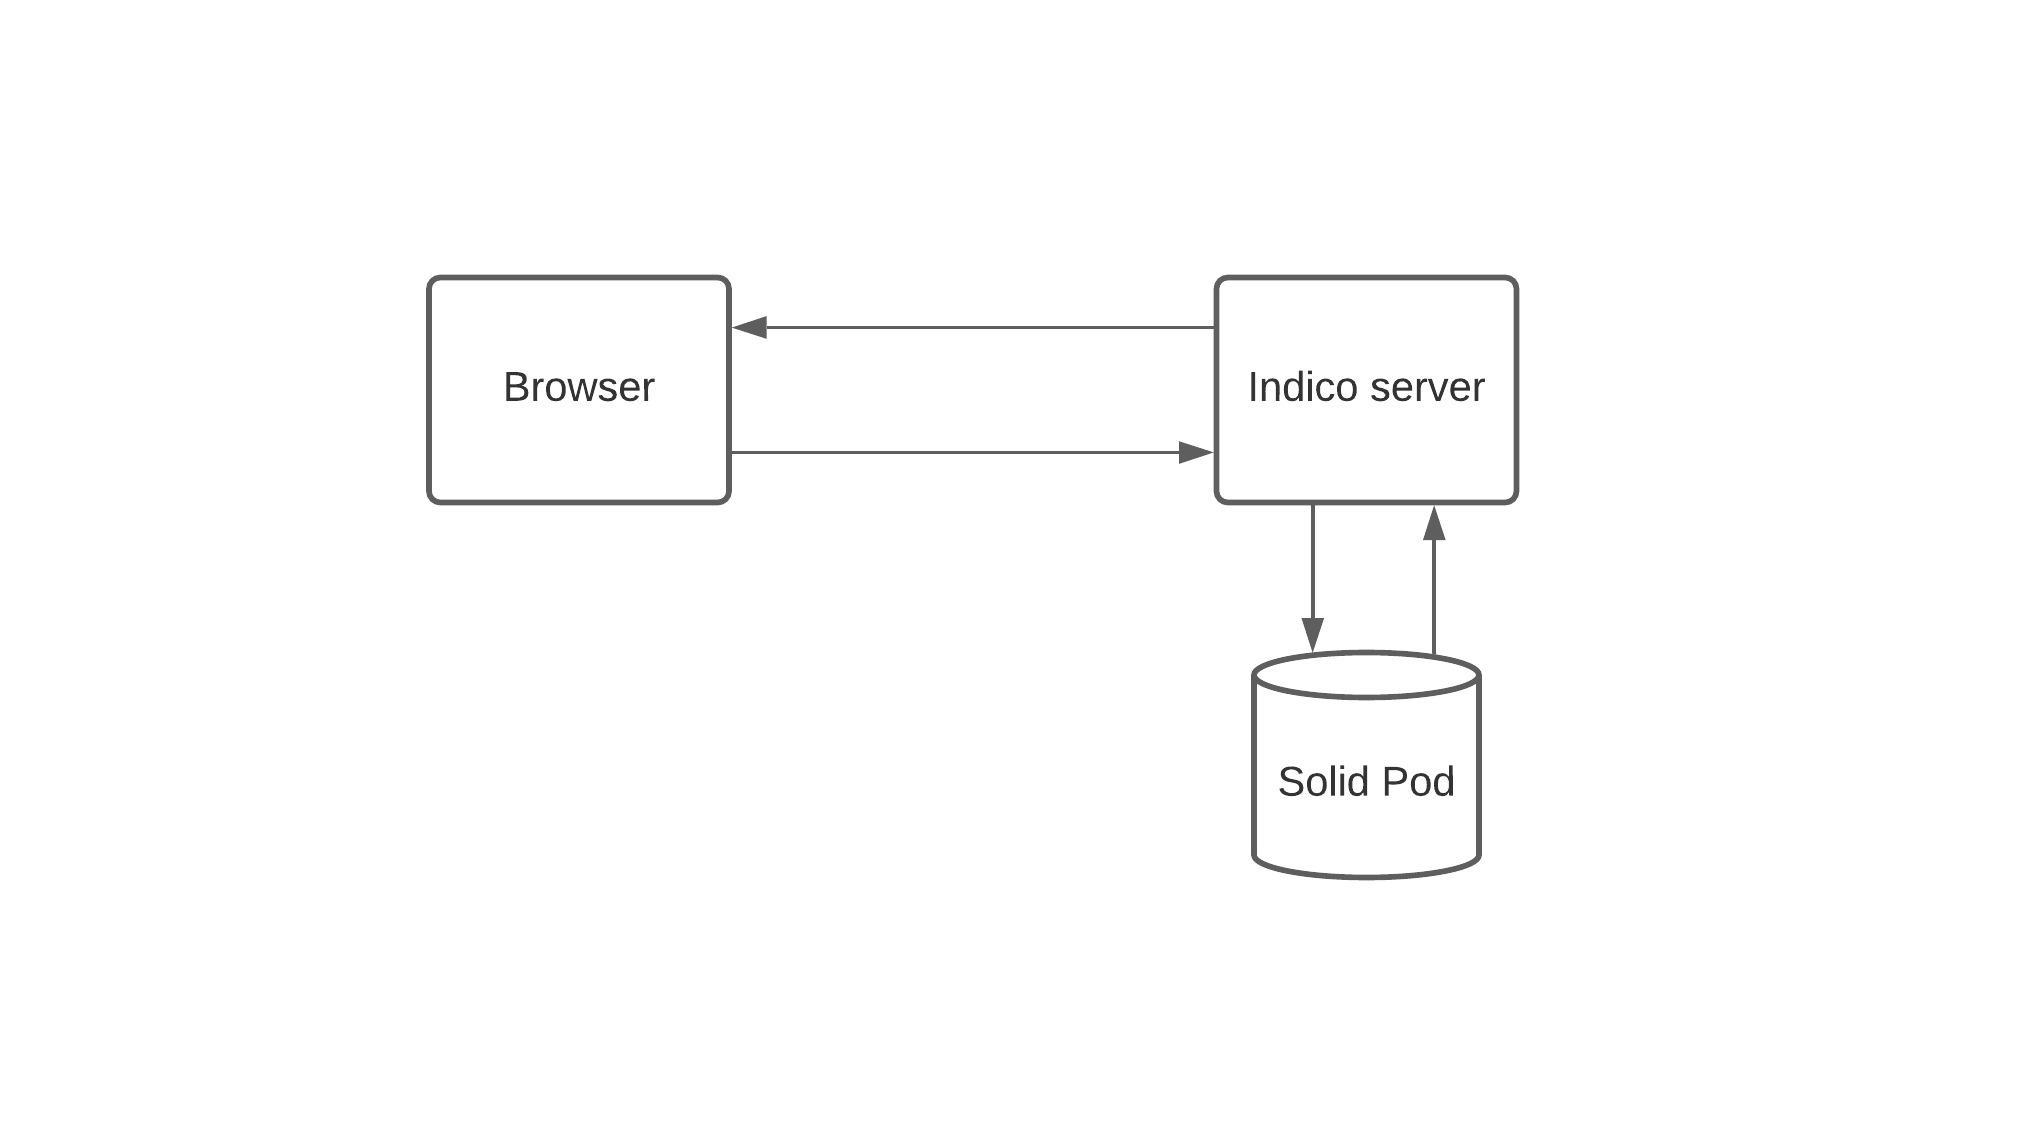
\includegraphics[width=0.8\textwidth]{prototype/graphs/poc-infrastructure-backend.jpeg}
    \caption{poc-infrastructure-backend}
    \label{fig:poc-infrastructure-backend}
\end{figure}


\begin{figure}
    \centering
    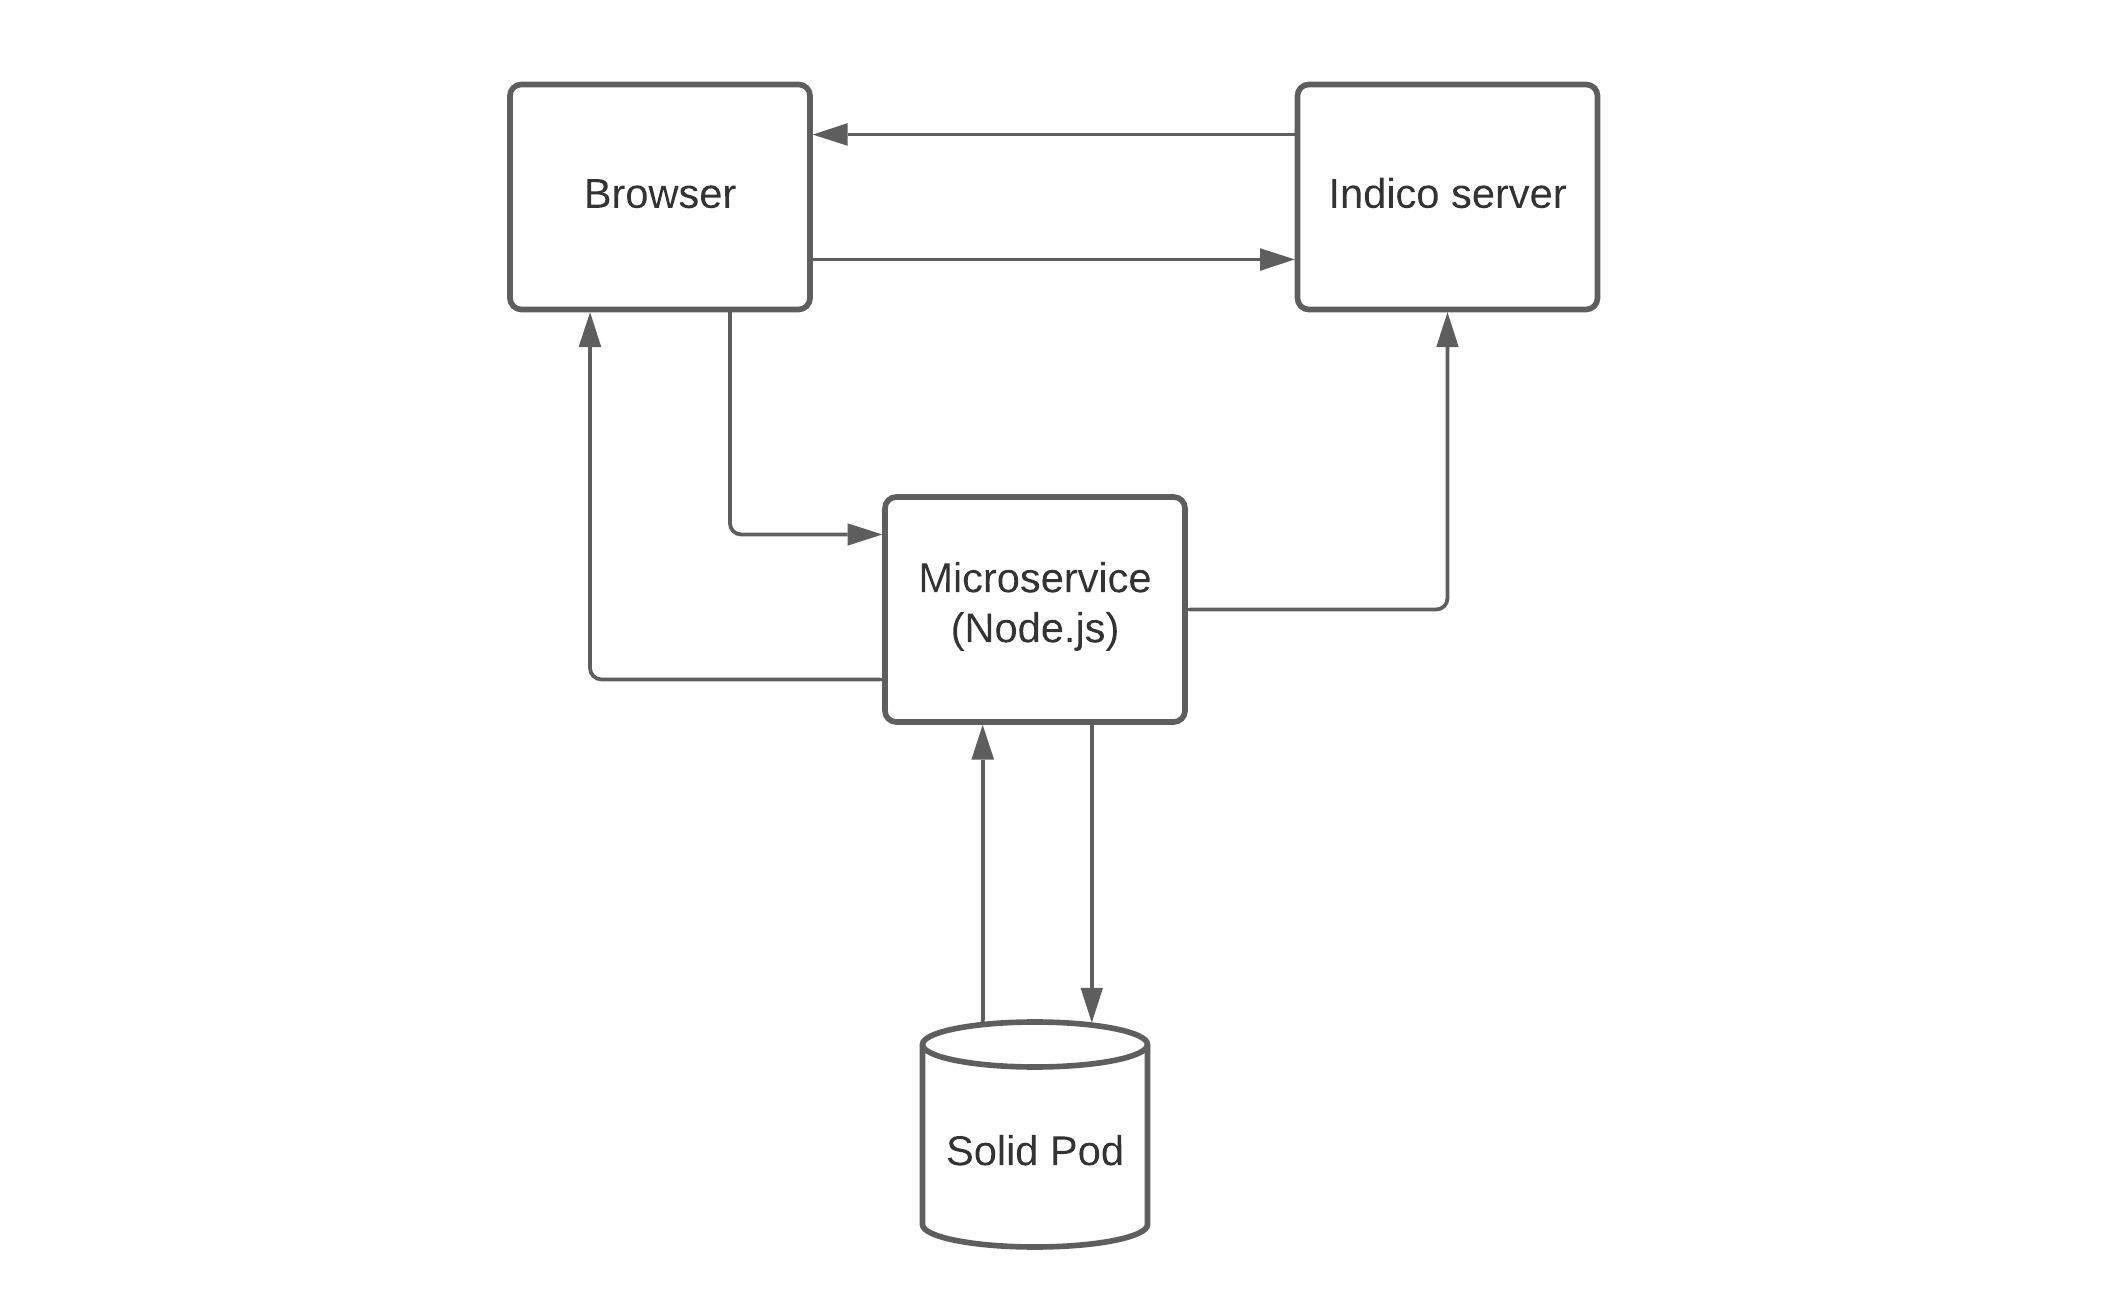
\includegraphics[width=0.8\textwidth]{prototype/graphs/poc-infrastructure-microservice.jpeg}
    \caption{poc-infrastructure-microservice}
    \label{fig:poc-infrastructure-microservice}
\end{figure}


\paragraph{Protection on Resource}\mbox{}\\

\paragraph{Modification of Resource from Pod}\mbox{}\\

\paragraph{Mitigation of Spam}\mbox{}\\

\paragraph{Giving Application Full Control of Pod}\mbox{}\\

\subsubsection{Integration with Indico}

\paragraph{Storing Reference to Comments in Indico}

\paragraph{Enforce Authenticated Session for Posting Comments}


\subsubsection{Evaluation}

\paragraph{System Description}
\paragraph{Context Diagram}
\paragraph{Stakeholders}
\paragraph{Drivers}
\paragraph{Metrics}
\paragraph{Levels}
\paragraph{Components}

\subsubsection{Analysis}

\subsection{POC 2: Auto-Complete for Conference Registration in Indico}

\subsubsection{Design}

TODO:
1st iteration, save data in pod
2nd iteration, only pull data from pod

\paragraph{Modification of Resource from Pod}

\paragraph{Payment on Input Fields}

\paragraph{Performance of Large Conference}

\paragraph{Availability of Crucial User Data}

\subsubsection{Integration with Indico}

\paragraph{Bind to Dynamically Created Form}

\subsubsection{Evaluation}

\paragraph{System Description}
\paragraph{Context Diagram}
\paragraph{Stakeholders}
\paragraph{Drivers}
\paragraph{Metrics}
\paragraph{Levels}
\paragraph{Components}

\subsubsection{Analysis}

\subsection{Deployment of Indico Instance}
